%CHAPTER 3 FROM HERE
%Please add \usepackage{tikz} to main.tex
%\usepackage{tikz}
%Please add a lstnewenvironment for computer shell:
%\lstnewenvironment{terminal}{\lstset{basicstyle=\footnotesize\ttfamily,
%		columns=flexible,
%		breaklines=true,
%		numbers=left,
%		%stepsize=1,
%		numberstyle=\tiny,
%		backgroundcolor=\color[rgb]{.7,.7,.7}}}{}

\chapter{Programming concepts for data analysis}

This chapter introduces readers to the basics of programming. It outlines how to install the software (R and Python) used in this book, explains how to deal with objects, statements, expressions, variables and different types of data, and shows how to create and understand simple control structures in object-based languages, such as loops and conditions.

\section{Installing R and Python}

In the previous chapter we had fun with data using the provided docker, which meant that there were very few things to install in order to run the initial examples. However, if you want to enjoy all the power of computational analysis of communication you must be able to install from scratch all the necessary software, packages and dependencies in order to complete your first steps as a programmer and then be able to write, adapt and run code. Nowadays you may find many online and cloud services that provide web interfaces to run code, both in R and Python, which might result useful depending on your needs. Nevertheless, we encourage you to install on your local computer all the basic software and packages that we will use throughout this book and that you will likely use in the near future in order to apply the learned techniques in your own research.  

As we already justified in the introduction of this book, R and Python are the most popular programming languages that data scientists and computational scholars have adopted to conduct their work.  Now, we should download and install these open-source and free applications in our local computers and become familiar with some additional resources -such as the popular \emph{integrated development environment} (IDEs) or the notebooks- that are widely spread for a more friendly interaction with coding. All the resources are typically available for MacOS, Windows and Linux, but keep in mind that their implementation in each operating system might differ (for example, in the way you install the software or when writing the absolute or relative paths in the code). 

Firstly, we will install R and its most popular IDE RStudio, and we will learn how to install additional packages and run a script. Remember that R is an object-based programming language orientated to statistical computing that will be useful in most of the stages of computational analysis of communication.  If you are completely new to this software but familiar with other popular statistical packages in social sciences (such as SPSS or STATA) you will find that you can performance in R many already-known statistical operations but within a different environment. If you are not familiar with other statistical packages, do not panic, we will guide you from the very beginning. Probably, the first thing you have to be aware of when installing R is that unlike many traditional software that require just one complete and initial installation, when working with R we will first install the raw programming language and then we will keep on installing additional components during all of our journey. It might sound cumbersome, but in fact it will make your work more powerful and flexible, since you will be able to choose the best way to interact with R and especially you will select the packages that are suitable for your project.
Now, let's install R. You can go the official R webpage\footnote{https://www.r-project.org}, where you will find lots of valuable information about the environment as well as the necessary documentation for working in R.  There are different versions of R, since there is a global community of developers that help to improve the software every year. You should go the CRAN mirrors and click onto any mirror (or the one you consider more close to your place of work). Within the mirror you can download the version you need depending of your operating system (figure~\ref{fig:cran}). In case you're not familiar with terms “CRAN” or “mirror”, the first refers to the \textit{Comprehensive R Archive Network}, which is an online repository of R packages; and the second, to the server where a copy of any package is available for download.

\begin{figure}
\centering
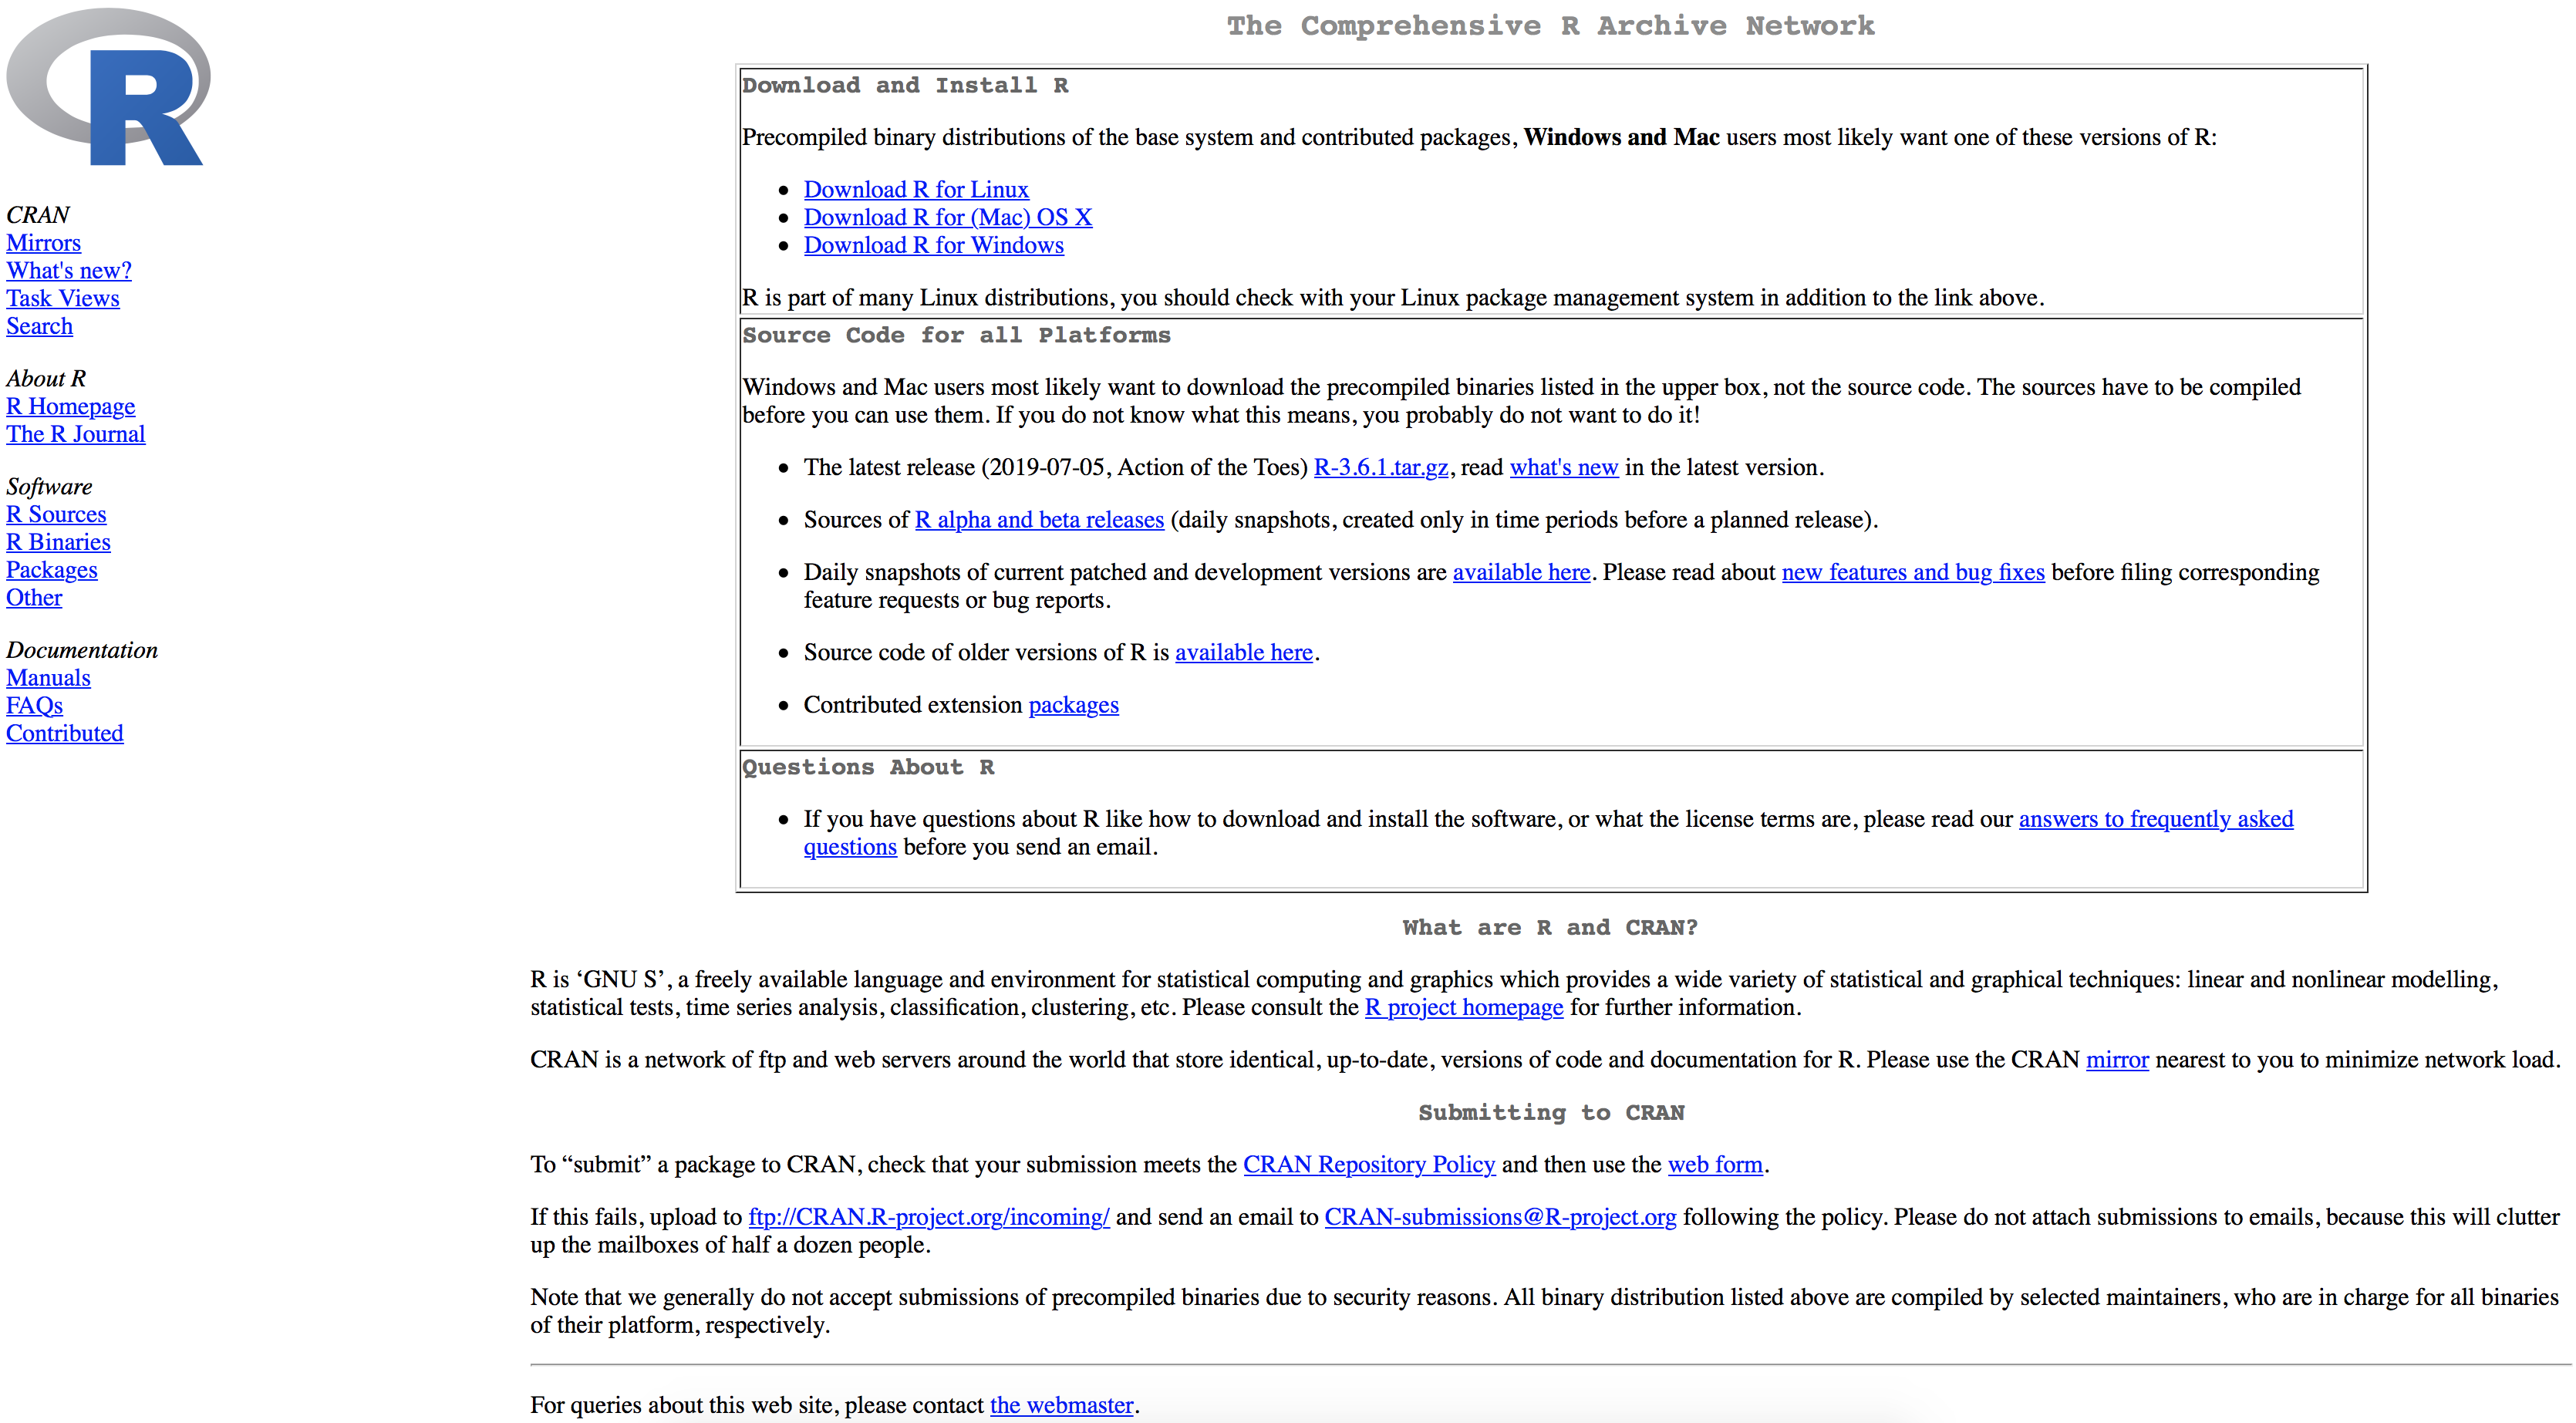
\includegraphics[width=0.9\linewidth]{figures/ch3_cran}
\caption{The Comprehensive R Archive Network.}
\label{fig:cran}
\end{figure}

Once you have downloaded and installed R on your computer (please follow the instructions on the page for each operating system), you will be able to open an R console (figure~\ref{fig:r_console}), where you can perform all operations in this programming language, from reading datasets to execute sophisticated data analysis. If you are new to computer science jargon, it is worthy to clarify what a \textit{console} is and what is the difference with a \textit{script} written in a document. A console is a text or graphical terminal where you write and execute commands. In fact, all computers and operating systems have terminals or consoles, which help us to interact with the machine, from listing files of a given folder (e.g. command \textit{ls} in Linux /MacOS) to install software, apps or utilities (e.g. command \textit{brew} in Linux/MacOS). The point is that any console is an active tool that normally executes the line or group of lines after you push the \textit{enter} button. This means that if you want to work with a more complex set of code lines such any \textit{script}, you may wish to write and test them in a separate file that you can save and also run from the console. This distinction is very useful in R, as you will normally work with both, an R document and an R console, in order to run your computation.

\begin{figure}
\centering
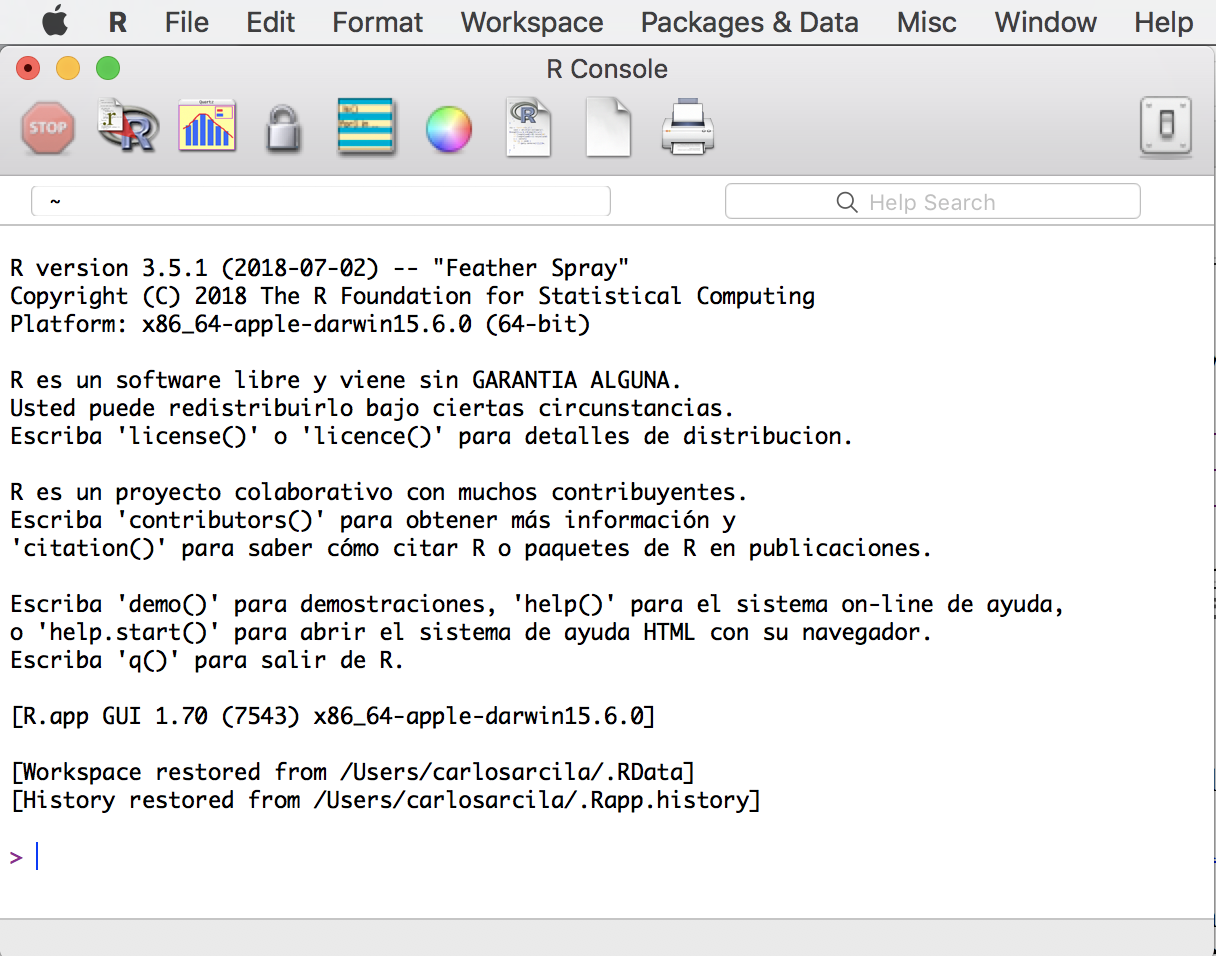
\includegraphics[width=0.9\linewidth]{figures/ch3_r_console}
\caption{R Console.}
\label{fig:r_console}
\end{figure}

\newcommand*{\icon}{
\includegraphics[scale=0.8]{figures/document_icon}}%
\newcommand*{\doc}{
\includegraphics[scale=0.7]{figures/r_document_icon}}%
\newcommand*{\rcom}{
\includegraphics[scale=0.8]{figures/r_icon}}%

In the R Console you will just have an empty line beginning with the sign \textgreater, where you can write any command, and also a menu with some useful icons. For example, the empty document icon \icon \  will allow you to create a new R document and write there your code. You can later use R document icon \doc \ to modify any given script or the general R icon \rcom \ to run the script or to load data in R. On the upper menu you will also find convenient tools such as Workspace or Packages \& Data. On one hand, remember that R is an object-orientated programming language, which means that all operations are performed with objects that we create or import, from simple variables to complex recursive functions. If you create an object \emph{x} with the value 17 (x \textless- 17), this object will be uploaded to RAM memory so you can call it every time you type \emph{x}.  Well, the menu Workspace will let you know which objects have been uploaded to this virtual space. We will go back to this issue later in this chapter when we discuss statements, expressions, variables, functions and methods. On the other hand, as we mentioned earlier, R can perform thousands of statistical operations with its raw language, but one of its greatest advantages is that we can use existing packages (also called libraries) that others have created to simplify our coding and to expand our possibilities in data analysis. You can find these packages in the CRAN, ensuring that there has been a minimum set of verification steps for that code, or directly from a developer webpage or repository. The menu Packages \& Data will help you to manage and install packages, as well as to load pre-existing data (freely available datasets we can work with). 

If you are unfamiliar with dealing with datasets in a coding environment, probably the first package you will be willing to install is R Commander\footnote{https://cran.r-project.org/web/packages/Rcmdr/index.html}, or Rcmdr for short, which is a graphical user interface for R that helps you to interact with data in a more visual way, similar to SPSS.	 You can install this package either by using the R Package Installer tool (Menu \textgreater Packages \& Data \textgreater Package Installer), or by typing the next syntax on your R Console:

\begin{exampler}
install.packages("Rcmdr", dependencies=TRUE)
\end{exampler}

Be patient, it will take some time to download and install on your local computer all the files and dependencies necessary to run R Commander. The good thing is that you have run your first line of code and you will notice that it is not that difficult; most of the commands you will use will follow a similar logic. In this case you have a native command (install) with a module (packages) and an argument ("Rcmdr") with an option (dependencies=TRUE). It is worth mentioning that once you have installed any package on your computer, you have to “call” it in the R environment every time you are going to work with it. This means that you have to indicate either on your R console or R Document, which libraries you will be using, so the program can load the package. The are two common methods to load or attach an add-on package: require() and library(). require() will return an error if the package is not installed. Whenever you want to know more about a method you can call for documentation using the ? symbol:

\begin{exampler}
?require	
\end{exampler}

Now, let’s load R Commander by typing:

\begin{exampler}
require(Rcmdr)
\end{exampler}

In this case, by loading Rcmdr a pop-up window will be displayed with the graphical interface to work with data and run basic statistics. In most of the cases, no window will show up, but the package will be loaded in the backend so you can use all its functions. For example, if we are working a on an R document (.r) where we write a set of instructions that need any particular package we should call that package in the file before it performs any operation included in it (by just entering a line such as:

\begin{terminal}
library(<the_package>)
\end{terminal}

With this line you ensure that you will not get an error message warning you that certain function does not exist or has not been properly called when your are running the script.

Now that you have learned how to install R and its packages on your computer, we should move on to get familiar with additional resources that are of great help when working with R. In particular we introduce RStudio, which is an IDE, free of charge and open source that will make our computational journey with R much more friendly and easier. Among many other advantages, in this environment you will have a workspace where you can simultaneously visualize your R documents (.r files), the R console, the objects or variables you load to memory and files or packages you are dealing with. You can find a desktop application that will run locally on your computer (RStudio Desktop) or a web-server version that you can install on a remote server and run from any web browser via Internet (RStudio Server). If it is your first time on this environment, we encourage you to download and install RStudio Desktop (figure~\ref{fig:r_studio}) from its official website\footnote{https://www.rstudio.com/products/rstudio/download/}. As in the case of R, please choose the appropriate installation file for your operating system (MacOS, Windows, Linux) and get the latest version.

\begin{figure}
\centering
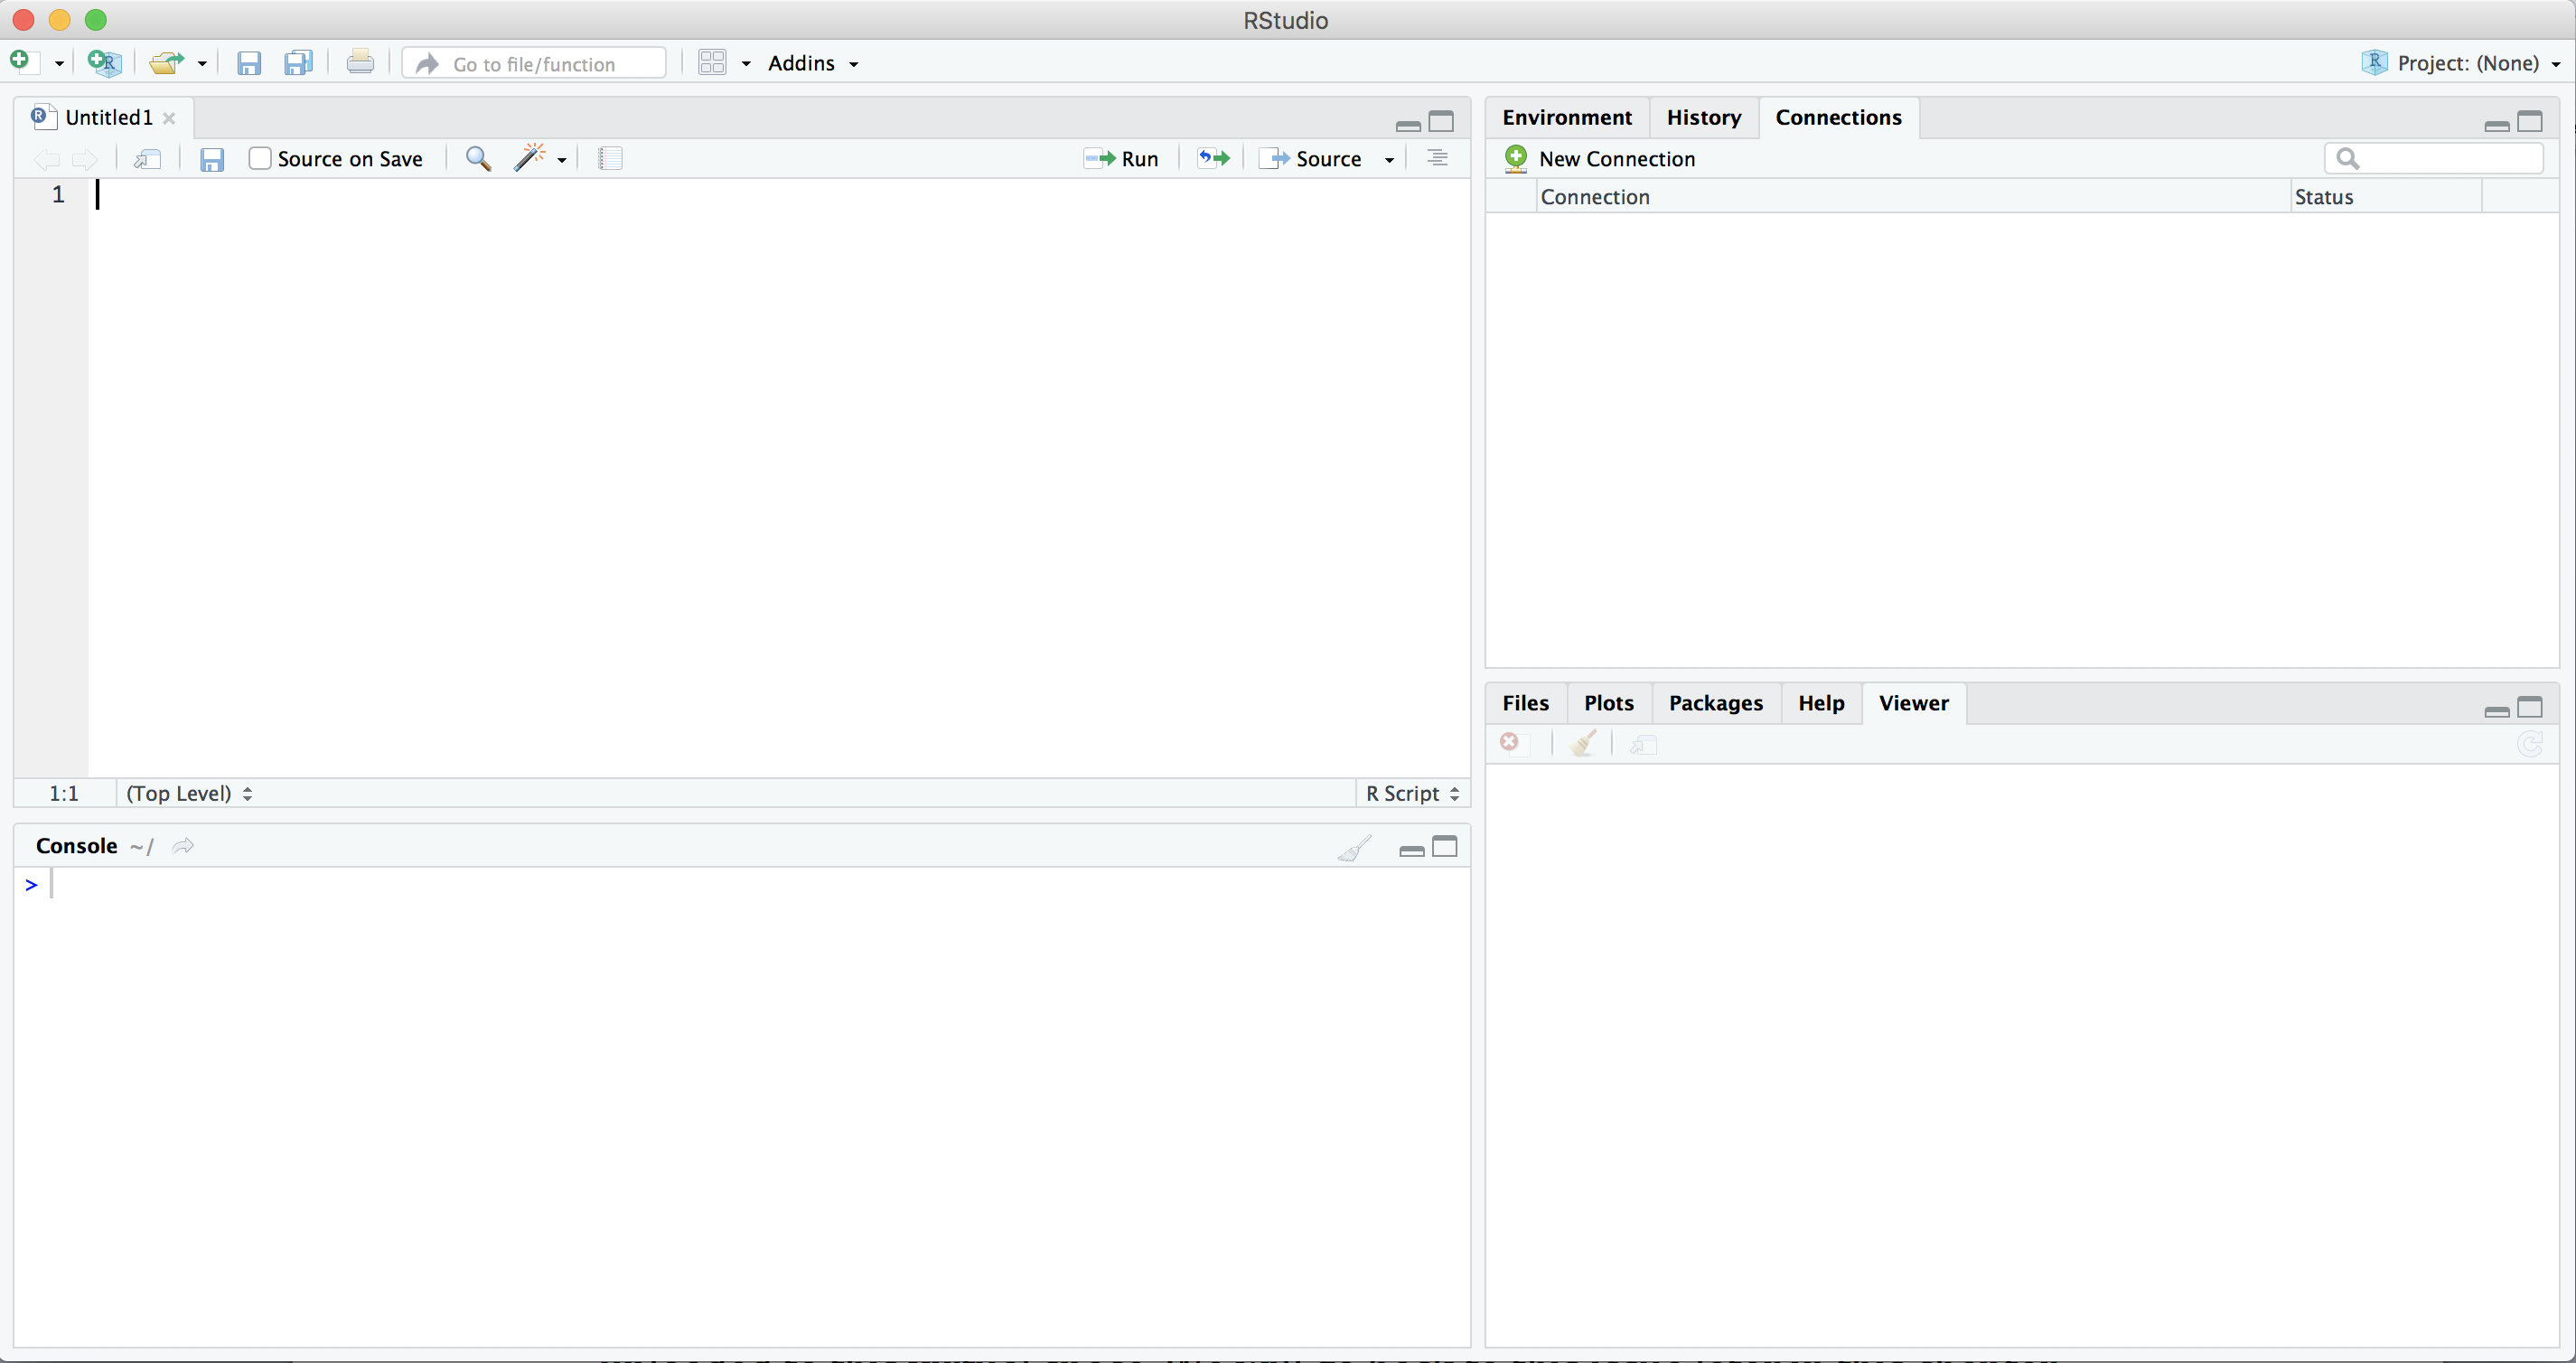
\includegraphics[width=0.9\linewidth]{figures/ch3_r_studio}
\caption{RStudio Desktop.}
\label{fig:r_studio}
\end{figure}

In RStudio you will see by default four main integrated windows (you may later reconfigure it), and the upper menu. In the up-left window, you can visualize and edit all the files you will work with, in special R documents (.r), data, and R Markdown documents (.rmd).  If it is the first time you hear about Markdown, keep this format in mind because it is a markup language for plain text that will help you to work with reproducible R documents based on a very simple syntax and ready-to-export to most universal formats such as HTML or PDF. The down-left window is the R console where you can directly write a syntax or where your will get the outcome from the code you have written and run in the R document. Please look at the up-left window and notice that there is a button named \textit{run}, which you will often use. By selecting partial or total lines of code in your script and clicking on this button you will execute the code and get the results in the console.  As you will realize with the first practices, it will be very useful to have the script in one window and gradually run parts of the code, instead of executing the whole document at once or to run it line by line in the console.

In the right side of RStudio workspace you will find two additional windows. In the up-right window there are three tabs. You will mostly use \textit{environment} and \textit{history}, and seldom \textit{connection} (just to connect to existing data sources such as those from ODBC or Spark). In \textit{environment} you can manage your workspace (the set of elements you need to deploy for data analysis) and have a list of the objects you have uploaded to it. You may also import datasets with this tool, and most importantly, you can save your workspace or open a previous one. In \textit{history} you will have an inventory of code executions, which you can save to a file, or move directly to console or to an R document. In the down-right window you will have five more useful tabs. In \textit{files} you can explore your computer and manage all the files you may use for the project, including importing datasets. In \textit{plots}, \textit{help} and \textit{viewer}, you can visualize the outputs figures, documentation and general outcomes, respectively, that you have executed in your script. Finally, the tab for \textit{packages} will be of great utility since it will let you install or update packages from CRAN or even from a file saved on your computer with a friendly interface.

Now that you have installed R and RStudio, let's change to Python. As most computational scientists do, we will jump from one application to another throughout this book, so do not worry if you have to wear two hats the same day, even at the very same time! The first thing will be to install Python on your local computer (though some operating systems come already with it as a default). As explained in chapter [INTRODUCTION], Python is an object-orientated programming language and it is probably the favourite language of computational and data scientists in all disciplines around the world. There are different releases of Python, but you will usually find a distinction between versions of Python 2 and those of Python 3, since some syntax and functions change from one to another. In this book, we will explain Python 3.x and all our examples and exercises will be written for this version. Notice that you might install different versions of Python on your local computer, and also create specific virtual environments (including a Python version and all its libraries and dependencies).  By doing this, you will be able to run any version depending on your needs. Thus, if you do not have already Python on your computer	\footnote{There are different ways to check if you already have it. For example, if you are in MacOS, you can open your system terminal and type \textit{python} –V or \textit{python --version}, and you will get a message with the version that is working by default in your computer or that has been set as an environment variable. There might be different versions already installed, so you might check directly for them: \textit{python2 --version} of \textit{python3 --version}.}, the first thing will be to download it and install it from its official webpage\footnote{https://www.python.org/downloads/}, selecting the right software according to your operating system (Windows, Linux/UNIX, Mac OS X).

During the installation, you will be informed that some additional features will be installed along with Python: normally an \textit{integrated development environment} (IDLE), \textit{Pip install packages} (pip) and \textit{documentation}. The IDLE will be very useful since it will provide you with a basic interface to work with Python files (.py) and the Python console. pip is a basic package that will help you to install and manage more software packages within Python. And documentation will provide you with basic help to work in this programming language.  In addition, you might be questioned if you want to add Python to path, which means that you set the \textit{path variable} in order to call the executable software from your \textit{system terminal} just by typing the word 'python'. We recommend selecting this option.  If you have never worked before with the system terminal of your computer, probably this is a good opportunity to know what and where it is. With this terminal you can interact with your machine and navigate through your files, create new ones, install programs, execute scripts, etc.  Everything you already do in your friendly and graphic interface in Windows, MacOS or LINUX, but performing it only with commands and code. Well, if you already downloaded and installed Python, you may open your system terminal\footnote{The terminal will look slightly different depending on your operating system. In MacOS or LINUX you can find it the 'Terminal' in the Utilities folder in Applications; and in Windows you can get the 'Command Prompt' in the Accessories folder in the All Programs menu.}  and launch Python from it! First, type \textit{python –V} and push enter to check your current installed version and then just type \textit{python} and you will open the software from the very same system terminal:

\begin{terminal}
python -V
python
\end{terminal}

\begin{figure}
\centering
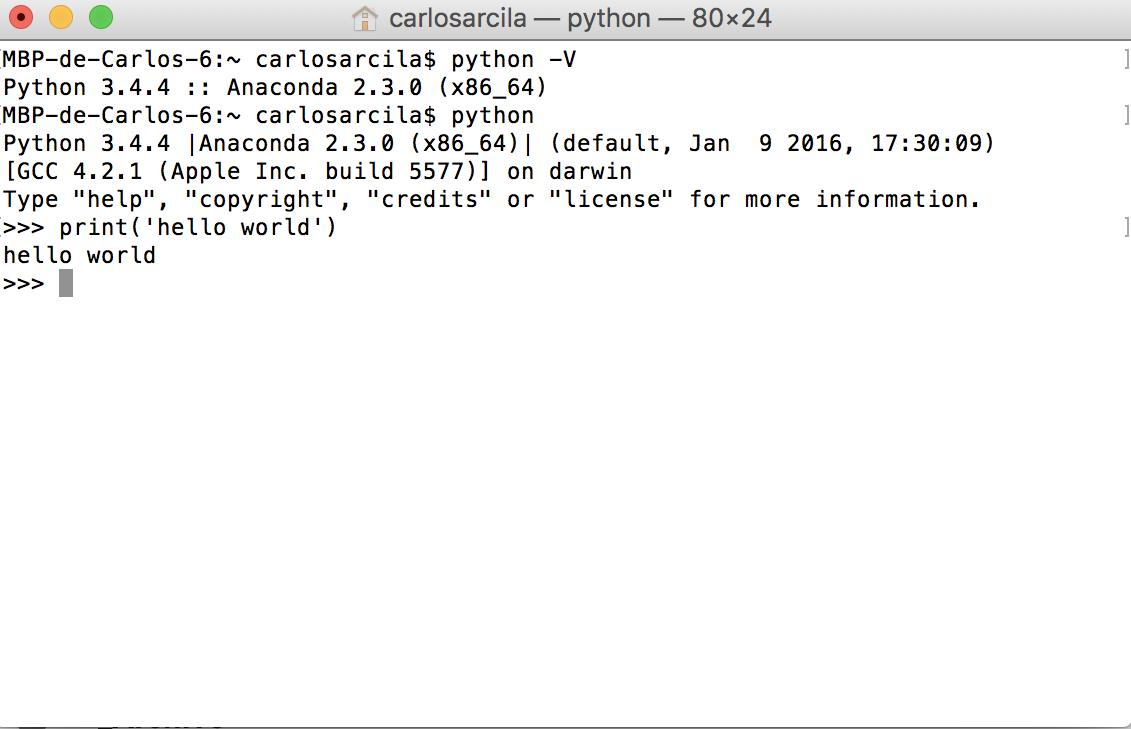
\includegraphics[width=0.9\linewidth]{figures/ch3_python_from_terminal}
\caption{Python launched from the Terminal.}
\label{fig:python_from_terminal}
\end{figure}

So, welcome to Python. You are now in the Python console, from where you freely operate this programming language. As it is a console, every line of code you type will be executed by pushing enter onto your keyboard, which means that if you have complex code you will mostly prefer to write the script in a Python file (.py) or similar (i.e. a notebook) and then run this file. However, as a first exercise it will be worth to keep the Python console open and write your first line of code on it, using the native function print:

\begin{examplepy}
print('hello world')
\end{examplepy}

Then, after running this line, you will get your first result or output (figure~\ref{fig:python_from_terminal}), which will be to display on the screen a sequence of characters, called a \textit{string}. You might say to your colleagues that you have written your first computer program, just as many computer scientists have done so in their first programming class. We will come back to coding in Python in the next sections. Now, let’s try to install some packages. Remember, that similar to R, in Python we can build every function from scratch, but there are many libraries or packages that will make our life easier, and some times, even more fun. There are different ways of installing a new package in Python, but the most classical one is by using the command pip from your system terminal. In order to quit the Python console and return to the system terminal, just type \textit{exit()} and push enter:

\begin{terminal}
exit()
\end{terminal}

Once in the terminal again you can use pip to install any package under your default python version (notice that if you have different versions or environments of Python, the package will not be installed in all of them).  In the last versions of Python some packages such as \textit{numpy} (for computing large multi-dimensional arrays and matrices) will be included  by default, but most likely you will need to install many others.  This is the case of \textit{tweepy}, which is a library to connect to the API's of Twitter and we will work with it in chapter [SCRAPING ONLINE DATA]. To install this package just run the next line on your system terminal:

\begin{terminal}
pip install tweepy
\end{terminal}

With this simple command, you will download and install this powerful package on your computer. You may try to check if you can now use the package, just by going again to Python console and use the command import to bring the library to your current session:

\begin{examplepy}
import tweepy
\end{examplepy}

If not error is showed, you can be happy that you successfully installed your first package in Python in just few seconds, using the system terminal and the raw Python software. Far beyond this basic environment, you might find more functionalities and shortcuts in this programming language if you use additional resources, such as any IDE or notebook, which will help you to interact with Python. In this book, we will mention three IDEs (IDLE, PyCharm and Spyder) and one notebook (Jupyter Notebook). IDLE (\textit{integrated development learning environment}) is a specific IDE provided for Python and which you might have already installed when you downloaded Python. IDLE has Python console (\textit{shell}) where you can directly write and execute code, and will also allow you to create Python files (.py) in a document-like window with some basic functionalities at the time of writing, such a colouring the code (depending on their function in the script), easy indentation or code debugging (figure~\ref{fig:python_idle}).  This will make your journey easier and more productive. 

\begin{figure}
\centering
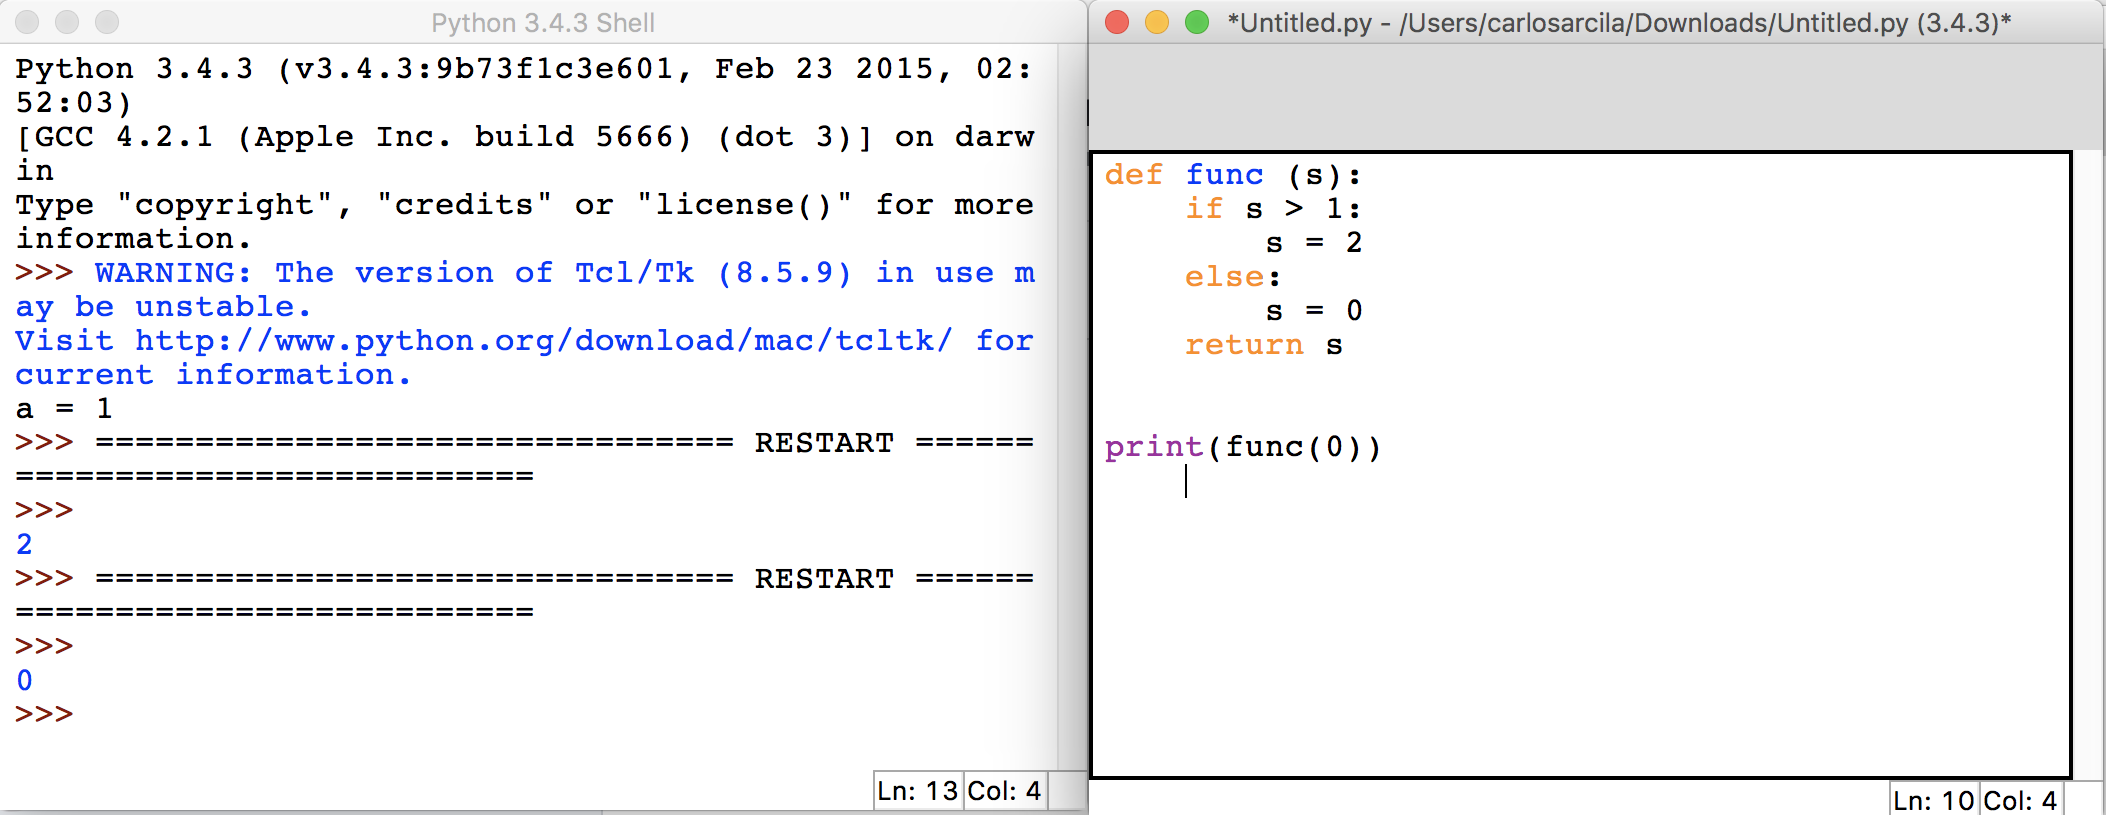
\includegraphics[width=0.9\linewidth]{figures/ch3_python_idle}
\caption{Python shell (left) and file (right) in IDLE.}
\label{fig:python_idle}
\end{figure}

The next useful IDE is PyCharm, which provides an even more graphical and integrated interface to deal with Python.  Developed by JetBrains, PyCharm has a free and open source \textit{Community} version that you can download and install on your local computer from its webpage\footnote{https://www.jetbrains.com/pycharm/download/} with options for 	Windows, MacOS and Linux. Once installed you can connect the software to any of the already installed versions of Python or even easily create \textit{virtual environments} to work on your projects. These virtual environments are isolated Python environments that will let you have a specific configuration and dependencies to work with in a project. For example, you may create one with an older version of Python, including specific releases of libraries.  You can equally achieve this with the pip command from your system terminal:

\begin{terminal}
pip install virtualenv
\end{terminal} 
 
BUT, PyCharm will help you to manage it with a graphical and friendly interface. The same happens with installing packages: using the \textit{Project} sub-menu from the \textit{Preferences} menu, you can install, update and delete any package related to any version of Python or virtual environment. In fact, easily dealing with Python versions and libraries is one of the main reasons why we recommend to new \textit{pythoners} to use PyCharm. But there are even more advantages.

Just like RStudio, PyCharm is an integrated interface that shows us different adjustable windows with a unique frame that we create for every project we open. Every time you create a project you have to name it, save it to a specific location (a folder where all your files will be stored) and choose an interpreter (a Python version or environment used by default in the project). Once created, you can begin to work on it with three main windows or sub-frames (figure~\ref{fig:pycharm}). The upper-left window contains the project structure and files. You can easily create or import folders and files and then navigate through them in this area. For example, by clicking on the right button of your mouse (or by going to File \textgreater New) you can create a new Python file (i.e. my\_first\_script.py) and organize your scripts by folders. In the upper-right window you will be able to visualize and modify the editable files contained in a project. All the open files will be in this window and you can access to any of them by clicking on its name situated in the upper tabs. In the low window you will find the output space as well as the Python and system consoles. This separation is very useful since you can work on your .py script (also with colour, indentation and error detection facilities), run it (from the \textit{Run} Menu) and produce the expected output in a separate window within the same frame.

\begin{figure}
\centering
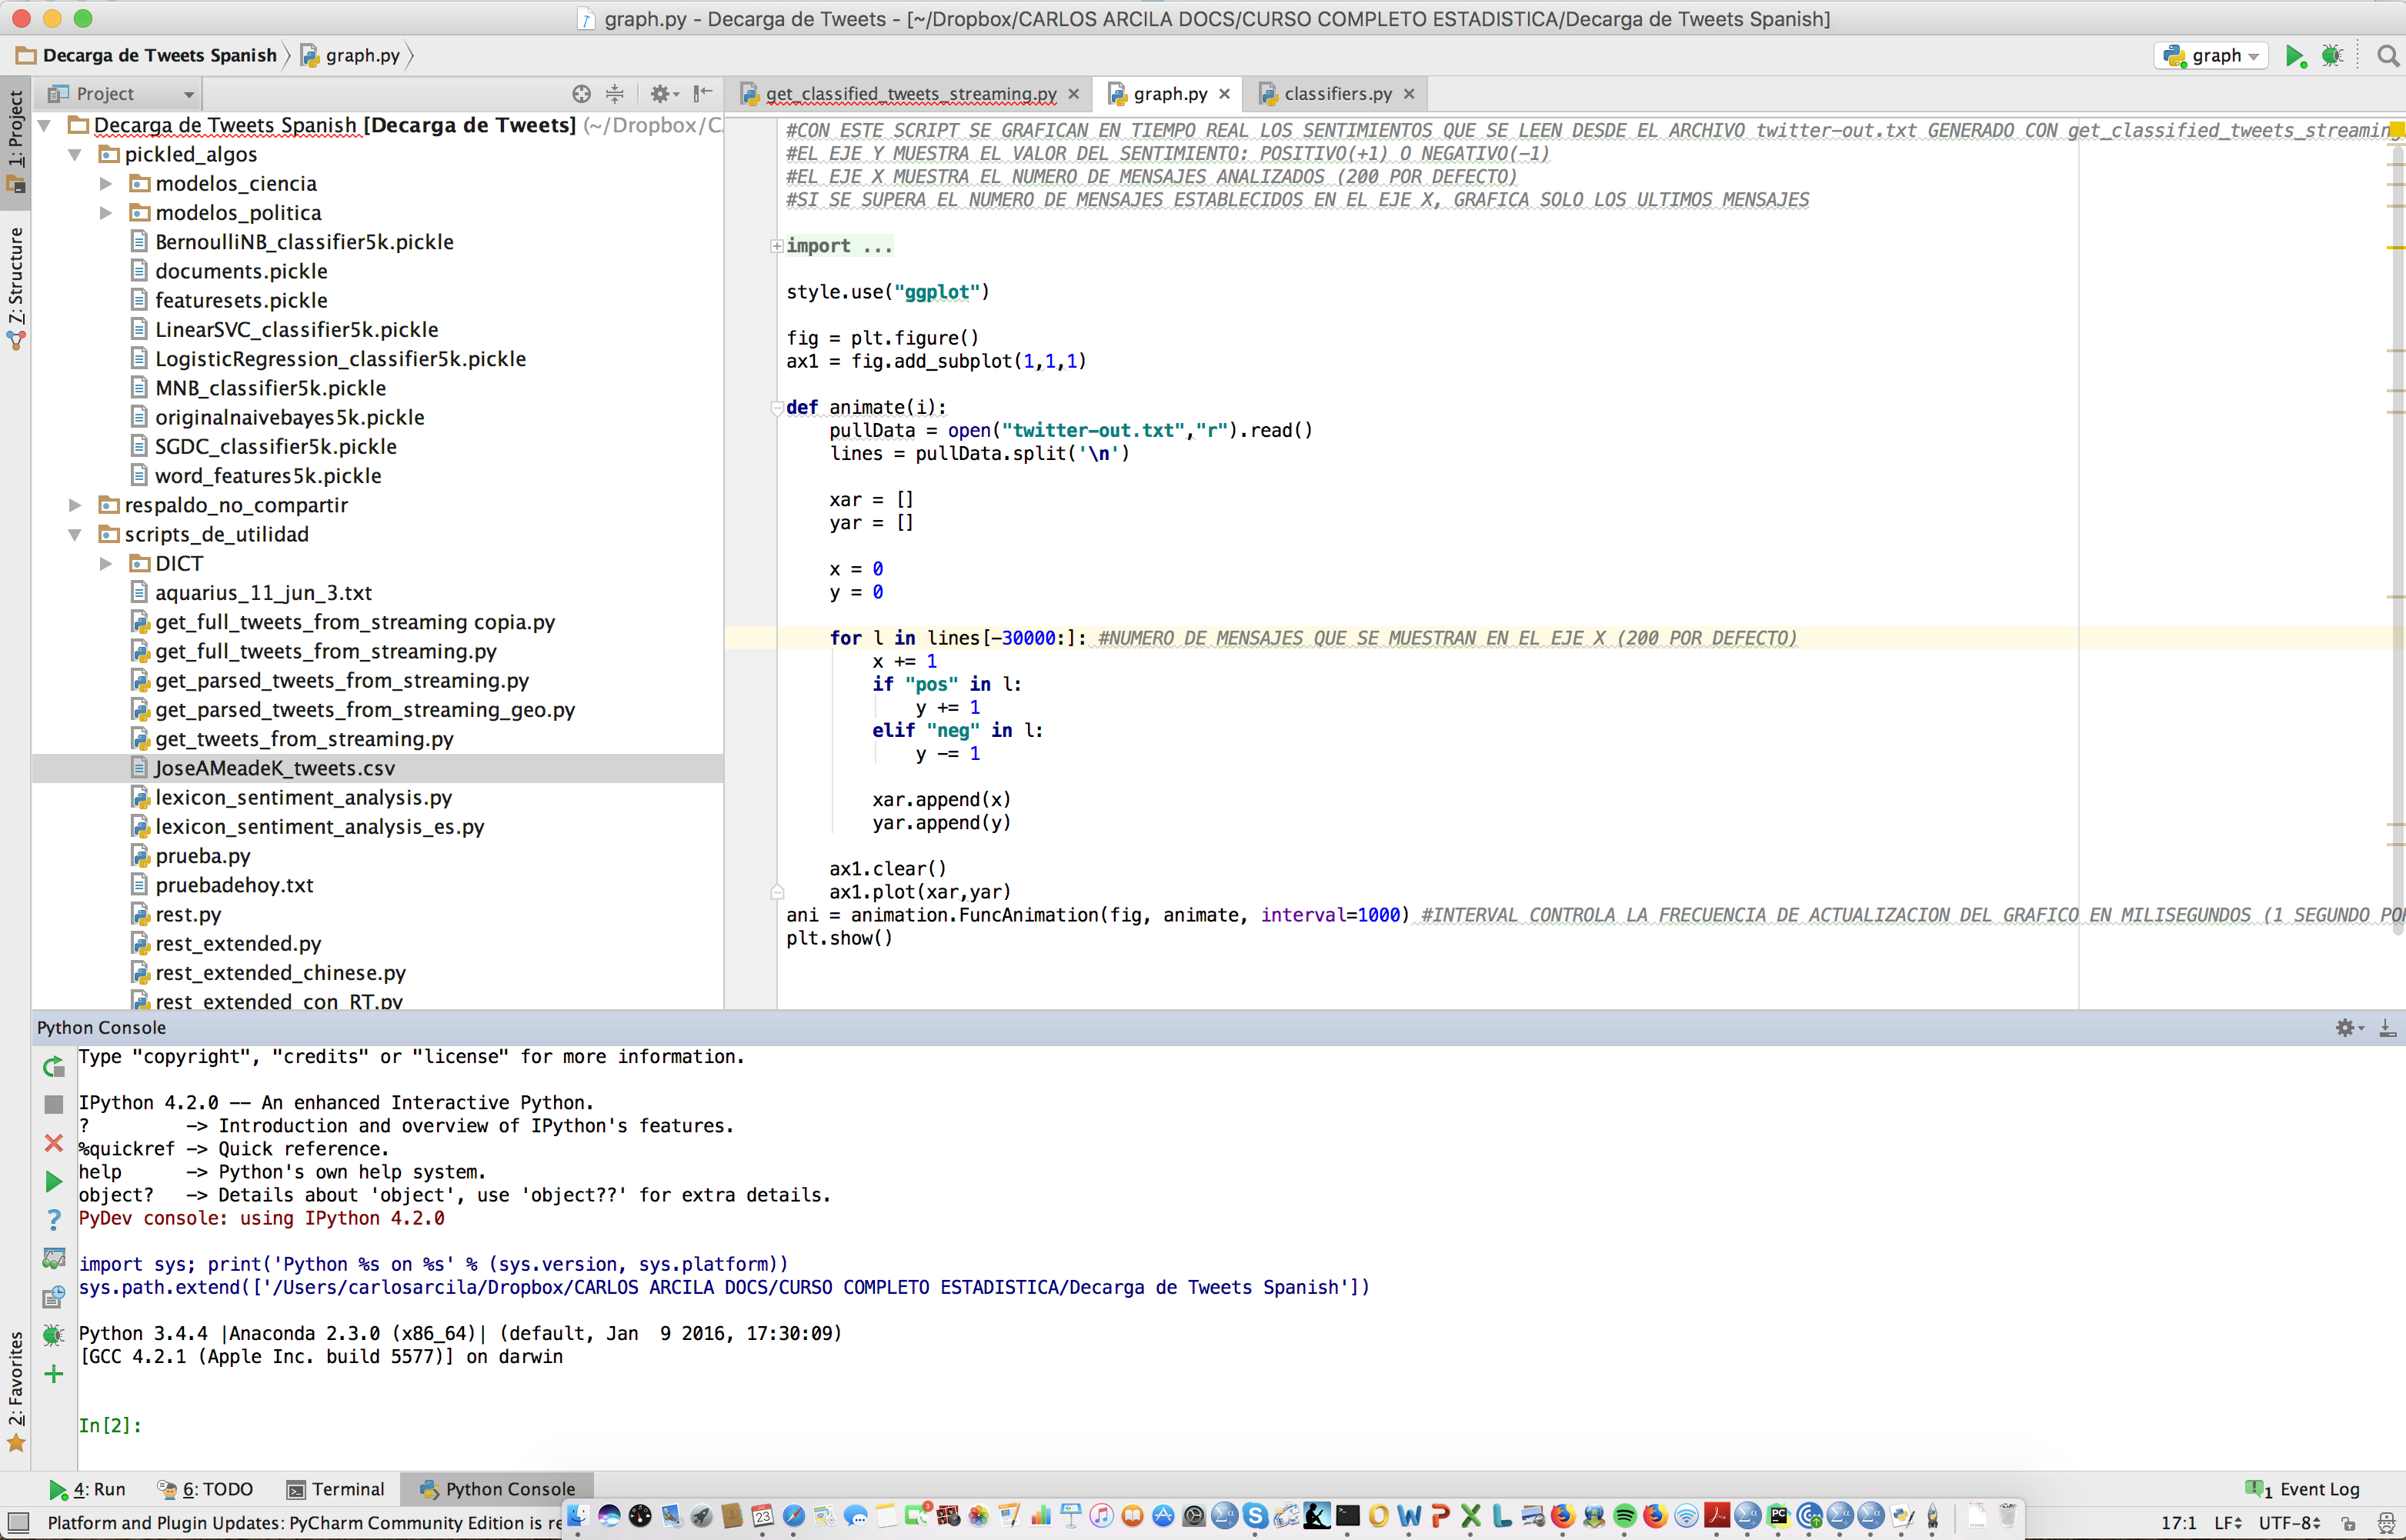
\includegraphics[width=0.9\linewidth]{figures/ch3_pycharm}
\caption{PyCharm environment.}
\label{fig:pycharm}
\end{figure}

The next two extra tools we would like you to familiarize with are Spyder and Jupyter Notebook. Spyder is an IDE for Python (pretty similar to PyCharm with a file editor and a console, but including a variable inspector) and Jupyter Notebook (included in the interactive development environment JupyterLab) is a web application that allows you to create and share documents that contain live code and text (and also equations and visualizations).  One of the nicest things of the Jupyter Notebook is that the code is inserted in fields that you can run one by one, getting its respective output, which added to the designed narrative text will make your script more clean and reproducible. Both, Spyder and Jupyter Notebook, are nowadays contained into the so called Anaconda Distribution, which you have probably heard about and that is one of the most used and extended platforms to perform data science. Anaconda is free and open-source, and is conceived to run Python and R code for data analysis and machine learning. This is a great tool for computational scientists and if you plan to follow this book we recommend you to install the complete Anaconda Distribution on your computer\footnote{https://www.anaconda.com/distribution/\#download-section}. In addition to Spyder and Jupyter Notebooks (and RStudio!), you will also get a set of pre-installed packages often used in data science (Pandas, Numpy, Scipy, Numba, Dask, Boreh, HoloViews, Datashader, Matplotlib, ScikitLearn, TensorFlow, etc.). Moreover, it will include the wonderful package Conda, which is an environment management system that will help you to install and update other libraries or dependencies. Once Anaconda is installed, you may say that you have on your local machine the most important software to perform computational analysis of communication. In the next chapter, we will address notebooks again as a good practice for a computational scientist.

\section{About variables and data types}

Now that you have all the necessary software in you own computer we can move on to the very basics of programming in R and Python\footnote{If you have not installed the require software yet and still want to follow this chapter, you may use available online platforms for RStudio (https://rstudio.cloud/) and Python (https://www.python.org/shell/).}.  Remember that both programming languages are object-orientated, which means that we normally have to create an object, upload it into the workspace and operate with it. Simplifying all technical details behind it, we might say that an object is any data structure that has some attributes and methods. You can think of an object as a classical variable you will work with, or as a function you need to store for later deployment. Every time you create an object and upload it into the workspace, you can call it back to see its value by just typing its name in the R or Python consoles; or if your are in IDE's such as RStudio or Sypder you can go to a window where there is a list of all uploaded objects or variables, their types and values.  In fact, creating an object in R and Python is extremely easy using the operators \textless- or =, respectively. We have to distinguish between objects and classes. A class is a blueprint or a prototype for an object, meaning that you include in a class a set of attributes that will characterize any object created or initiated from that class. As a matter of simplicity we will focus first on creating and understanding objects themselves and later in this section we will briefly explain how create a class. 

Let's begin again with R.  As a statistical programming language, R users need to deal with different types of data and perform multiple operations with them. R supports a variety of data types that include: vectors (numeric, character, logical, etc.), lists, matrices, arrays, factors and data frames. For those first-time programmers with knowledge of software such as SPSS or Excel (where you normally only deal with a data frame of rows and columns), this might sound to be a little bit annoying, but in fact it will give much more control on your data analysis process and, in general, on your computational approach. For a very nice and complete explanation of data types in R check  the book by Field, Miles \& Field~\cite{field2012discovering}, but for this book we need to be sure you understand the fundamentals in order to continue to the next chapters. 

First, think of the \emph{vector object} as the basic data type.  There are six types of these atomic vectors: numeric, integer, complex, character, logical and raw. Imagine you want to begin by storing a single numeric value as an object called x\emph{a} with the value of 100. Go to your R console and type:

\begin{exampler}
a <- 100
print(class(a))
\end{exampler}

The first line is mandatory to create the object \emph{a} and store its value 100; and the second is illustrative and will give you the class of the created object, in this case "numeric". Notice that we are using two native functions of R, \emph{print} and \emph{class}, and including \emph{a} as an argument of \emph{class}, and the very same \emph{class(a)} as an argument of \emph{print}. This is the way we work in object-orientated programming and if you compare to other languages you will realize that is a very simple syntax indeed. Once created, you can now perform multiple operations with \emph{a} and other values or new variables. For example, you could transform \emph{a} by multiplying \emph{a} by 2, create a new variable \emph{b} of value 50 and then create another new object \emph{c} with the result \emph{a} + \emph{b}:

\begin{exampler}
a <- a * 2
b <- 50
c <- a + b
print(c)
\end{exampler}

You will get a new numeric vector object \emph{c} of value 250. And this is the way you will mostly operate with data when working with R. Notice that so far you have only used numeric vector objects, but we have some more. Numerics support floats numbers (i.e. 20.5) as well as integers (i.e. 20), however if you want to limit your object to just integers you can change its class just by adding \emph{L} to the number when creating the variable. Same if you want to work with a complex numeric object that includes some declared variable and/or formulae, you just create such object with the internal variables and operators. Let’s see both cases:

\begin{exampler}
d <- 20L
print(class(i))
e <- 100+50x
print(class(e))
\end{exampler}

As a computational analyst of communication you will usually work with text objects or string of characters, which are called character vector objects in R, and you can create them just by adding single or double quotes to the value of the variable. Just think of a tweet or a Facebook post that you want to load into your workspace for natural language processing analysis:

\begin{exampler}
tweet <- "I am happy learning R!!!"
print(class(tweet))
\end{exampler}

There are two more types. First, the raw object produces raw bytes from string of characters and is created just by adding the command \emph{charToRaw} before the object. The second is the logical object, which stores a basic constant such as TRUE or FALSE. Here you can see how to create them:

\begin{exampler}
raw_string <- charToRaw("Any text")
print(class(v raw_string))
logical_operator <- TRUE 
print(class(logical_operator))
\end{exampler}

Take into account that you can easily operate two numeric objects or one numeric with one integer, but there might be some restrictions when putting together two different types of data, such as multiplying a character by a number. Table~\ref{tab:vector_objects} summarizes all these initial data types.

\begin{table}[ht]
\label{tab:vector_objects}
\caption{Classes of vector objects in R}
\centering
\begin{tabular}{c c c p{2cm}}
\hline\hline
Data type & Example & Code \\ [0.5ex]
\hline
Numeric&1, 2.5, 100, 2500.38& a\textless- 100 \\
Integer&20L, 100L&d\textless- 20L \\
Complex& 100+50x, 8*3i &e\textless- 100+50x \\
Character&   \parbox[t]{4cm}{\centering 'a', "I am happy learning R!!!", "200", 'R', "FALSE"} & tweet \textless- "I am happy learning R!!!" \\
Raw& \parbox[t]{4cm}{\centering "Any text" stored as:  41 6e 79 20 74 65 78 74} & raw\_string \textless- charToRaw("Any text") \\
Logical& TRUE, FALSE & logical\_operator \textless- TRUE  \\ [1ex]
\hline
\end{tabular}
\label{table:nonlin}
\end{table}

Thus, by bringing together a set of same-class vector objects we can create a vector. A vector is a basic structure of R and holds different elements of the same type (numeric, integer, complex, character, logical, raw) in a one-dimensional array.	You will use vectors very often to run computation and we can easily create them using the c() function. For example, we can create a numeric vector with the scores of a class of 10 students or a character vector of three countries:

\begin{exampler}
scores <- c(8, 8, 7, 6, 9, 4, 9, 2, 8, 5)
class(scores)
countries <- c('Netherlands', 'Germany', 'Spain')
class(countries)
\end{exampler}
 
As you see, the data types will correspond to only one class, either numeric or character, since vectors contain only one class. If we create the vector with two different data types, R will recognize one class forcing some elements to be transformed into the dominant class. For example, if you re-build the vector of scores (a new set of values will be loaded into the workspace) with a new student who has been graded with the letter \emph{b} instead of a number, your vector will become a character vector:

\begin{exampler}
scores <- c(8, 8, 7, 6, 9, 4, 9, 2, 8, 5,  'b')
class(scores)
print(scores)
\end{exampler}

Beyond the class (which is a powerful function because you can create new classes your self), you can also get the R internal type of the object (storage mode), using the typeof() function:

\begin{exampler}
typeof(scores)
\end{exampler}

Having a vector means that you can operate with it in many ways. The basic is \emph{indexing}, which is a technique that you will use with other data types (list, arrays, matrices, data frames) and in other languages such as Python.  Indexing helps you to locate any given element or group of elements within a vector using its or their positions. In R all positions begin in the number 1 (you will see that in Python and other languages they will begin on 0) and you can index using the square brackets [] over the vector:

\begin{exampler}
scores[11]
scores[1, 10]
scores[1:10]
\end{exampler}

In the first case, we asked for the score of the 11th student ("b"); in the second we asked for the 1st and 10th position ("8"  "5"); and finally for all the elements between the 1st and 10th position ("8" "8" "7" "6" "9" "4" "9" "2" "8" "5"). As the vector was forced to be a string, all the elements –even numeric- are now characters. Indexing is very useful to access elements and also to create new objects from a part of another one. Imagine you want to create a new numeric vector by \emph{slicing} the vector scores with just the numeric values and change its class using the function as.numeric:

\begin{exampler}
scores2 <- as.numeric(scores[1:10])
typeof(scores2)
\end{exampler}

And voilà, we have a new object called scores2 with the original values of the vector scores and of type \emph{double} (double precision floating point numbers, which is equivalent to the class numeric).  We can do many other things like adding a value to an existing vector or creating a vector from scratch by using a function. In the first case, you can include the new numeric score of 7 (imagine we translate the grade \emph{b} to the number 7) to our vector by any of the two following procedures:

\begin{exampler}
c(scores2, 7)
\end{exampler}

or

\begin{exampler}
append(scores2, 7)
\end{exampler}

If you want to be sure that the new values are correctly loaded into your workspace, you should apply any of these operations to the vary object:

\begin{exampler}
scores2 <- c(scores2, 7)
\end{exampler}

or

\begin{exampler}
scores2 <- append(scores2, 7)
\end{exampler}

Same in case you want to remove an element from your vector. For dropping the 11th student's score recently included you just index negatively the value of the vector:

\begin{exampler}
scores2 <- scores2[-11]
\end{exampler}

For the second case, we might wish to create a vector from an operator or a function, without typing each value. Using the operator ':', we can create numeric vectors with a range of numbers, from 1 to 20 or from -5 to 5:	

\begin{exampler}
range1 <- 1:20
range2 <- -5:5
\end{exampler}

On the other hand, you can use a function to create more complex vectors. For example the function seq() will help you to generate regular sequences by providing the number of points of an interval.  Imagine you want to create a numeric vector than begins in point 0 and finishes in point 1, including all possible values that separate those two points by a step of 0.2. Let's create that vector and check the amount of created elements by using the function length:

\begin{exampler}
my_sequence <- seq(0,1, by=0.2)
length(my_sequence)
\end{exampler}

So far, we have focused on vectors, but there are more data types in R (lists, matrices, arrays, factors, data frames). Now that you have a clear idea of what vector objects and indexing are, and that you have the basics to create and operate with vectors, it will be much easier to understand the other data types. The first R-object that you must be familiar with is the list, which is similar to vectors but may contain different type of elements, functions and even other lists. We create lists in a similar way to vectors, except that we have to add the word \emph{list} before declaring the values. Let's build a list with four different kind of elements, a numeric object, a character object, a square root function (sqrt) and a numeric vector:

\begin{exampler}
my_list <- list(33, 'Twitter', sqrt, c(1,2,3,4))
class(my_list)
\end{exampler}

You can check this is a list of four elements and you can use any of these elements (even the function to get the square root of 16!) using the indexing:

\begin{exampler}
length(my_sentence)
my_list[[3]](16)
\end{exampler}

Matrices are two-dimensional rectangular data sets that include values in rows and columns. This is the kind of data you will have to deal with in many analyses shown in this book, such as those related to machine learning.  To create a matrix in R you have to use the function "matrix" and create a vector of values with the indication of how many rows and columns will be on it. We also have to tell R if the order of the values is determined by the row or not.  Let’s create a simple matrix of 0 and 1’s, and check its shape by using the dimension function:

\begin{exampler}
my_matrix <- matrix( c(0,0,1,1,0,1), nrow = 2, ncol = 3, byrow = TRUE)
dim(my_matrix)
\end{exampler}

Create a new matrix (my\_matrix2) and repeat the above code typing FALSE in the byrow argument and you will better understand how it changes the values of the matrix, even when the shape (2x3) remains identical. As you may cleverly imagine, we can operate with matrices, such as adding up two of them:

\begin{exampler}
my_matrix + my_matrix2
\end{exampler}

Another powerful data type are the arrays, which might be similar to matrices but without the restriction of the two-dimensional rectangular space. This means that you create your own dimensions, indicating (in order) the number of rows, columns and matrices of the array. Your will need vectors as inputs and dimensions as parameters. For example, three-dimensional arrays are fundamental when writing pixel values and coding images.  By now, you can create a simple illustration of a 3D array:

\begin{exampler}
3d_array <- array(c('green', 'yellow', 'red'),dim = c(3,3,3))
dim(3d_array)
print(3d_array)
\end{exampler}

The next R-object is the factor, which might be very useful when working with categorical data. When dealing with factors, you can store the values of a vector with their corresponding labels, which in turn will produce levels. If you create a factor, it will automatically read the labels from the values of the vector, but you may manually change those levels. Let's see the next lines of code. The first line will create again a vector of scores of ten students. Then we automatically convert the vector into a factor (reading the very same values as labels) and finally we create the labels ("fail" or "pass") for each of the possible grades:

\begin{exampler}
scores <- c(8, 8, 7, 6, 9, 4, 9, 2, 8, 5)
factor_scores <- factor(scores)
factor_scores_2 <- factor(scores, levels = c(1,2,3,4,5,6,7,8,9,10), labels = c("fail", "fail", "fail", "fail", "fail", "pass", "pass", "pass", "pass", "pass"))
\end{exampler}

The factor-type object factor\_scores\_2 will be probably more useful to deal with a bigger amount of students. While we have only two levels (which can be identified with the function nlevels), we can have many values to connect with those labels.

Finally, we have the wonderful data frames. This is the friendly type of data that you find in SPSS or Excel that will help you in a wide range of statistical analysis (though in more advanced exercises such in machine learning you will not be able to use them any more!).  A data frame is a tabular data object that includes rows (usually the instances) and columns (the variables). In a three-column data frame, the first variable can be \emph{numeric}, the second \emph{character} and the third \emph{logic}, but the important thing is that each variable is a vector and that all these vectors must be of the same length. We create data frames from scratch using the data.frame() function.  Let’s generate a simple data frame of three instances (each case is an author of this book) and three variables of the types numeric (\emph{age}), character (\emph{country} where he obtained his master degree) and logic (\emph{living abroad}, weather he currently lives out of his born country). We will create the values of age and living abroad, but we will re-use the values of the above created character vector \emph{conutries} for this exercise:

\begin{exampler}
authors <- data.frame(age = c(38, 36, 39), countries, living_abroad= c(FALSE, TRUE, TRUE))
print(authors)
\end{exampler}

When you print the data frame, you will obtain something like this:

\begin{exampler}
  	age   	countries 		living_abroad
1 	 38 	Netherlands         	FALSE
2 	 36 	Germany         	TRUE
3 	 39    	Spain          		TRUE
\end{exampler}

Notice that you have the label of the variables at the top of each column and that it creates an automatic numbering for indexing the rows.  You will learn more about data frames and of all data types in chapter [DATA STRUCTURES], where we will also introduce you to some libraries to deal with different data structures. Now we have to move on to variables and data types in Python.

As an object-orientated language programming, Python allows us to create objects, variables or functions, and load them into its workspace. The fundamentals are the same of R, so if you correctly understood the last explanations you will find very easy to do the same in Python. However, keep in mind that you will probably have to develop more skills to master Python since this programming language is not constrained to statistics and is flexible for many more computational tasks, both at small and large scale. This means that its syntax might become more complex than R, even when you will not need to know all of it to run most of computational analysis of communication.  For a deeper and understandable reading of Python programming we recommend the book by M. Lutz\cite{lutz2013learning}. Nonetheless, in the next paragraphs we will introduce you to the variables and data types in Python, so you can easy follow the book and the proposed exercises.  

A good way to start is to understand the built-in object types in Python and how to operate with them. Similarly to R we have numeric, integer, complex, character and logical, which we will now call float, integer, complex, string and boolean, respectively. Objects will also include lists, tuples, sets, dictionaries, functions and classes. If you are missing vectors, arrays or matrices as objects, do not worry, even when they are not built-in objects in Python, we can create them using specialized libraries such as Numpy (see chapter [DATA STRUCTURES]). Now you can open your Python console and we can create our first objects and load them into our workspace. First, let’s create a couple of objects \emph{x} and \emph{yy} containing only numbers as values, and third object \emph{z} that contains the result of an arithmetic operation between those two:

\begin{examplepy}
x = 40
y = 512.23
z = x * y
\end{examplepy}

If we now use the native function \emph{type} we will get that \emph{x} is an integer and \emph{y} and \emph{z} floats:

\begin{examplepy}
type(x)
type(y)
type(z)
\end{examplepy}

So far it is pretty similar to R! You can now create a complex number, which takes two parameters: a real part and an imaginary part:

\begin{examplepy}
complex = complex(20 + 8i)
type(complex)
\end{examplepy}

We will deal a lot with character objects in English and other languages, for which we will use an object composed by a series of characters called string:

\begin{examplepy}
facebook_post = 'Hello mates! Does anyone find Python easier than R?'
type(facebook_post)
\end{examplepy}

Pretty similar to R we create logical objects, called Booleans in Python. Just notice that True or False values are case sensitive and while in R you must capitalize the whole value (TRUE, FALSE), in Python we only capitalize the first letter:

\begin{examplepy}
boolean = True
type(boolean)
\end{examplepy}

Lists are mutable sequences of different types of elements. In other words, they are ordered collections of objects with no fixed size. We build this Python object using square brackets [], instead of parentheses (), as we did in R. Pay attention to this detail because in Python we will create tuples if you use the parentheses. Tuples are similar to lists, except that they are immutable (which means that they are constant or unchangeable and you can not freely change their values, just as numbers or strings).  We can now create our first list and tuple, and get their sizes with the native function len:

\begin{examplepy}
my_list = [1, 0, -1, 'positive', 'neutral', 'negative']
len(my_list)
my_tuple = (1, 0, -1, 'positive', 'neutral', 'negative')
len(my_tuple)
\end{examplepy}
	
We have created two sequences of six objects (three integers and three strings) that represent common numeric and categorical values for sentiment analysis. The first sequence is a list and the second a tuple. We can get any value of the list or tuple by indexing its position, just keep in mind that indexing in Python begins in 0 and not in 1 like in R. Let's get the value 'neutral' in each:

\begin{examplepy}
my_list[4]
my_tuple[4]
\end{examplepy}

Imagine now that you decide – by any reason - that the value 'neutral' should be substituted by the value 'informative' in the created sequences. You can do it updating the object:

\begin{examplepy}
my_list[4] = 'informative'
my_tuple[4] = 'informative'
\end{examplepy}

The list will be correctly updated, but the code you run to change the tuple will give you an error (with some message such as: "'tuple' object does not support item assignment"). Thus, tuples are immutable and are worth for certain types of operations because they give stability to a particular computation. Notice that we can include any object into lists or tuples. For example, if we include a list into another list we create a nested list, which might be very useful for representing matrices or multi-dimensional arrays in Python:

\begin{examplepy}
matrix = [[1, 2, 3], [4, 5, 6], [7,8,9]] 
\end{examplepy}	

We also have another Python object called sets. A set is a mutable collection of \emph{unique} elements (you cannot repeat a value) with no order. As it is not properly ordered, you cannot run any indexing or slicing operation on it. The immutable version of sets are called frozensets:

\begin{examplepy}
colours = set(['blue', 'yellow', 'red'])
type(colours)
colours2 = frozenset(['blue', 'yellow', 'red'])
type(colours2)
\end{examplepy}

Finally, Python has dictionaries, another helpful object.	 Dictionaries contain unordered and mutable collections of objects that contain certain information in another object. Python generates this data type in form of { 'key' : \textless value \textgreater} in order to map any object by its key and not by its relative position in the collection. This means that you will index using the key. You will find dictionaries very useful in your journey as a computational scientist or practitioner, since they are flexible ways to store and retrieve structured information. We can create them using the curly brackets {} and including each key-value pair as an element of the collection:

\begin{examplepy}
sentiments = {"positive" : 1, "neutral" : 0, "negative" : -1}
type(sentiments)
\end{examplepy}

An advantage of the dictionaries is that you can create an open object and fill later its values. This is probably the way you will see dictionaries in code:

\begin{examplepy}
grades =  {}
grades['A'] = 4
grades['B'] = 3
grades['C'] = 2
grades['D'] = 1
print(grades)
\end{examplepy}

As in other objects you can index its elements, by keep in mind that you do it using the key and not the position in the sequences. For example, we want to get the values of the object 'positive' in the dictionary \emph{sentiments} and of the object 'A' in the dictionary \emph{grades}:

\begin{examplepy}
print(sentiments['positive'])
print(grades['A'])
\end{examplepy}

Now that you have gone through most types of objects in R and Python, we need to remember that objects are different from classes, as we mentioned at the beginning of this section. A class is a prototype with attributes that helps to build an object when it is created from that class. R has three class systems: S3 class, S4 class and Reference Class.  Imagine that we have some data of a news item that we want to convert to a class using the basic S3 class:

\begin{exampler}
news <- list(headline = "Scientists discover how to cure AIDS", date = 21012030, positive_tone = TRUE)
class(news) <- "news_piece"
\end{exampler}

Or using Reference Class:

\begin{exampler}
setRefClass("news_piece")
\end{exampler}

Then you have stored the information of the class news\_piece.  You can do this also with S4 class, which allows you to define the formal structure of the class:

\begin{exampler}
setClass("news_piece", slots=list(headline="character", date="numeric", positive_tone="logical"))
\end{exampler}

Using S4 class definition you can create a new object using the attributes of the created class, which is very useful to maintain consistency:

\begin{exampler}
news2 <- new("news_piece", headline="Thousands of new refugees run from hunger after war begins", date=22012030, positive_tone = FALSE)
\end{exampler}

On the contrary, Python has just a single class. We define the class in a similar way we will define functions (see next section). We use the keyword class and, in some cases, the built-in \_\_init\_\_() function.  Let's create a very single class in Python including a numeric object in the class and later using that class to define a new object:

\begin{examplepy}
class MyWeight:
...    	 x = 74
weigth = MyWeight()
print (weigth.x)
\end{examplepy}

As you see, we created the object \emph{weight} using the properties (x in this case) of the class MyWeight. This procedure is probably of limited use but good to illustrate what a class is in Python. A more interesting approach to create the class is using the \_\_init\_\_() function, which is a special function that assigns values to object properties and is executed when the class is being initiated. In simpler words, this function helps us to assign different values within the class, creating an internal structure that will be used when we create an object based on that class. You can run the next example on your Python console for a better understanding of the concept. Imagine you want to create the same class news\_piece we did in R and then use that class to create an object:

\begin{examplepy}
class news_piece:
...     def __init__(self, headline, date, positive_tone):
...             self.headline = headline
...             self.date = date
...             self.positive_tone = positive_tone
news2 = news_piece("Thousands of new refugees run from hunger after war begins", 22012030, False)
print(news2.headline)
\end{examplepy}

As you see, with the last line of the code we obtain a part of the created object (in this case the headline) based on the structure designed in the class news\_piece.

In the next section you will learn the basics of how to write code in R and Python.

\section{Simple control structures: loops and conditions}	

Having a clear understanding of what an object is allows us to comprehend how object-orientated languages such as R and Python work, but now we need to get some literacy of how to write code and interact with the computer using these programs. Learning a programming language is just like learning any new language.  Imagine you want to speak Italian or you want to learn how to play the piano. First thing will be to learn some words or musical notes, and to get familiarized with some examples or basic structures. This is what we have done so far in the last sections and chapters by providing real examples of computational analysis of communication and explaining you the main types of objects you will have to deal with in R and Python. In the case of Italian or piano, you would have to learn next some grammar: How to form sentences in different times or how play some accords and reproduce patterns, respectively. And this is exactly how we should now move on to acquiring computational literacy; by learning some rules to make the computer do exactly  what you want.

Remember that you can interact with R and Python directly on their consoles just by typing any given command on the shell. However, when you begin to use several of these commands and combine them with a specific syntax you will need to put all these instructions into a script that can run partially or entirely. Scripts are very useful as the syntax of our code becomes more complex and you move to many levels of \emph{indentation} (logical empty spaces - 2 in R and 4 in Pyhton - depicting blocks and sub-blocks on your code structure) that can result messy on a shell. Thus, to learn how to create functions and simple control structures you should create and save documents (i.e. .r or .py) that we call scripts. 

And this is the way computer programs work: you give them some \emph{statements} (directly or from a script) to which they react. Statements are just written instructions that are executed by the console.  We call a sequence of these statements a \emph{computer program} . In the previous section, when we created objects or \emph{variables} (i.e. a \textless- 100 or a = 100) we already dealt with the basic statement, which is called \emph{assignment statement}. But the statements can be more complex and include many internal components, such as \emph{assignment statement}, which are representations of values that combine variables, constants and functions (i.e.  x+1 AND z\textless100). There are some specific expressions (such as \emph{lists of comprehension} in Python) that we will discuss later, but for now you can notice that by using statements, expressions and variables you have the basics for computer programming.

Fortunately, we have great syntactic tools to write code. Both, R and Python have \emph{loops} and \emph{conditional statements}, which will make your coding journey much easier and with more sophisticated results because you can control the way your statements are executed. By controlling the flow of instructions you can deal with a lot of challenges in computer programming such as iterating over unlimited cases or executing part of your code as a function of new inputs. 

Firstly, loops are sequences that are executed once, indefinitely or until a certain condition is reached. This means that you can operate over a set of objects as many times as you want just by giving one instruction. The most common types of loops are \emph{for}, \emph{while} and \emph{repeat} (do-while). Let’s understand this concept by explaining the for-loops. Imagine you have a list of headlines as an object either on R or Python and you want simple code to print out the length of each message. Of course you can go headline by headline using the indexing, but you will get bored or will not have time enough if you have thousands of cases. Thus, the idea is to operate a loop in the list so you can get all the results, from the first until the last element, with just one instruction.  The syntax of the for-loop in R is:

\begin{exampler}
for (val in sequence)
{
statement
}
\end{exampler}

Now you can go to R and create a new R document and then run the whole next script to check how to get the number of characters of each headline, both by a manual procedure and by an automatic procedure using a for-loop:

\begin{exampler}
#This script creates in R a list of headlines and shows two ways to count the number of characters of each string
#The first way is manual 
headlines <- list ('US condemns South new terrorist  attacks', 'New elections forces UK to go back to the UE', 'Venezuelan president is dismissed') 
print('manual results:	')
print(nchar(headlines[1]))
print(nchar(headlines[2]))
print(nchar(headlines[3]))
#and the second is using a for-loop
print('for-loop results:')
for (x in headlines){
  print(nchar(x))
}
\end{exampler}

You can notice that you have same results, but with the loop you can automatize your operation writing few lines of code. As we will stress along this book, a good practice in coding is to be efficient and harmonious in the amount of code we write, which is another justification for using loops.  

In Python the syntax of the for-loop is:

\begin{examplepy}
for <var> in <iterable>:
    <statement(s)>
\end{examplepy}

Thus, you can go to Python and create a similar script, as the example below:

\begin{examplepy}
#This script creates in Python a list of headlines and shows two ways to count the number of characters of each string
#We create a list of headlines (strings):
headlines = ('US condemns South new terrorist  attacks', 'New elections forces UK to go back to the UE', 'Venezuelan president is dismissed') 
#The first way is manual:
print('manual results:')
print(len(headlines[0]))
print(len(headlines[1]))
print(len(headlines[2]))
#and the second is using a for-loop
print('for-loop results:')
for x in headlines:
    print(len(x))
\end{examplepy}

Another way to iterate in Python is using list comprehensions  (not available natively in R), which are a stylish way to create list of elements automatically even with conditional clauses. This is the syntax:

\begin{examplepy}
list  = [ expression for item in list if conditional ]
\end{examplepy}

To make a simple example (without any conditional clause), let's create a list with the number of characters of each headline by executing the next piece of code in your script:

\begin{examplepy}
#Another way to iterate is the list comprehensions
len_headlines= [len(x) for x in headlines]
print(len_headlines)
\end{examplepy}

Secondly, the conditional statements will allow you to control the flow and order of the statements written on your code. This means you can mandate the machine to do this or that, depending on a given circumstance. These statements use logic operators to test \emph{if} your condition is met (True) or not (False) and execute an instruction accordingly. Both, in R and Python, we use the clauses \emph{if}, \emph{else if} (\emph{elif} in Python) and \emph{else} to write the syntax of the conditional statements. Let's begin showing you the basic structure of the conditional statement in R:

\begin{exampler}
if (condition) {
    Statement1
} else {
    Statement2
}
\end{exampler}

Imagine you want to print the headlines of the above example only if the text is less than 40 characters long. We can include the conditional statement in the loop adding the next code to the script:

\begin{exampler}
#Print the headline if it is < 40 characters
for (x in headlines){
  if (nchar(x)<40) {
    print(x)}
  }
\end{exampler}

Or you could use the clause \emph{else} to return a missing value ('NaN') in all the cases that do not satisfy the condition of length:

\begin{exampler}
#Print the headline if it is < 40 characters and print 'NaN' in the other cases
for (x in headlines){
  if (nchar(x)<40) {
    print(x)}
  else 
    print ('NaN')}
\end{exampler}

The syntax in Python is even simpler:

\begin{examplepy}
#Print the headline if it is < 40 characters and print 'NaN' in the other cases
if condition_1:
    statement_1
elif condition_2:
    statement_2
else:
    statement_3
\end{examplepy}

Notice that we have included the clause \emph{elif} in the structure (in R it is noted \emph{else if}). \emph{elif} is just another clause which statement must be executed only if an earlier condition was not satisfied. However, the reasoning behind the logic operators remains the same. Now, let's re-write all our conditional-statement exercises and include them into the above created Python script:

\begin{examplepy}
#Print the headline if it is < 40 characters
for x in headlines:
  if len(x)<40:
    print(x)

#Print the headline if it is < 40 characters and print 'NaN' in the other cases
for x in headlines:
  if len(x)<40:
    print(x)
  else :
    print ('NaN')
\end{examplepy}

To finish this chapter, we will talk about \emph{functions} and \emph{methods}, which are fundamental concepts in writing code in object-orientated programming. Both are objects that we use to store a set of statements and operations that we can later use without writing the whole syntax again. This makes our code simpler and more powerful. These two concepts are similar, but the difference between them is that the functions are defined independently from the object, while methods are created based on a class, meaning that they are associated to an object. Methods and functions may include loops and conditionals, as well as any other operators.  We will illustrate how to create simple functions in R and Python, so you will have a better understating of how they work. Imagine you want to create two functions: one that computes the 60\% of any given number and another that estimates this percentage only if the given argument is above the threshold of 5. The structure of a function in R is:

\begin{exampler}
function_name <- function(arg_1, arg_2, ...) {
   Function body 
}
\end{exampler}

Thus we can write the next script in R to load and test these two simple functions:

\begin{exampler}
#This scripts in R creates two simple functions to estimate the 60% of any given number

#The first function computes the 60% always
por_60 <- function(x) {
  return(x*0.6) 
}
print (por_60(10))
print (por_60(4))

#The second function computes the 60% ONLY IF the argument is above 5, 
# and the other cases the function returns the very same argument

por_60_cond <- function(x) {
  if (x>5) {
    return(x*0.6)
  } else {
    return(x)
  }
}
print (por_60_cond(10))
print (por_60_cond(4))
\end{exampler}

Imagine that you have a list of 5 scores and you wish to apply the function por\_60\_cond to all the scores at once using a loop. Add these lines to your code:

\begin{exampler}
#Create the list with the scores and then apply a simple loop
scores <- list(3,4,5,6,7)
for (x in scores)
{
  print(por_60_cond(x))
}
\end{exampler}

Now, let’s see the structure of a function in Python:

\begin{examplepy}
def function_name(arg_1, arg_2, ...):
  statement
\end{examplepy}

And adapt the above script to Python:

\begin{examplepy}
#This script in Python creates two simple functions to estimate the 60% of any given number

#The first function computes the 60% always
def por_60(x):
  return x*0.6
print (por_60(10))
print (por_60(4))

#The second function computes the 60% ONLY IF the argument is above 5, 
# and the other cases the function returns the very same argument
def por_60_cond(x):
  if x>5:
    return x*0.6
  else:
    return x
print (por_60_cond(10))
print (por_60_cond(4))

#Create the list with the scores and then apply a simple loop
scores = (3,4,5,6,7)
for x in scores:
  print(por_60_cond(x))
\end{examplepy}

So far you have taken your first steps as a programmer, but there many more advanced things to learn that are out of the scope of this book. You can find a lot of literature, online documentation and even wonderful Youtube tutorials to keep learning. We can recommend the works by M. Crawley\cite{crawley2012r}  and J. VanderPlas\cite{vanderplas2016python}  to have more insights of R and Python, respectively. In the next chapter, we will get deeper into the world of code in order to learn how and why to re-use existing code, what to do if you are stock during your programming journey and what are the best practices when coding.